% -*- latex -*-
%%%%%%%%%%%%%%%%%%%%%%%%%%%%%%%%%%%%%%%%%%%%%%%%%%%%%%%%%%%%%%%%
%%%%%%%%%%%%%%%%%%%%%%%%%%%%%%%%%%%%%%%%%%%%%%%%%%%%%%%%%%%%%%%%
%%%%
%%%% This text file is part of the source of 
%%%% `Introduction to High-Performance Scientific Computing'
%%%% by Victor Eijkhout, copyright 2012-2022
%%%%
%%%% This book is distributed under a Creative Commons Attribution 3.0
%%%% Unported (CC BY 3.0) license and made possible by funding from
%%%% The Saylor Foundation \url{http://www.saylor.org}.
%%%%
%%%%
%%%%%%%%%%%%%%%%%%%%%%%%%%%%%%%%%%%%%%%%%%%%%%%%%%%%%%%%%%%%%%%%
%%%%%%%%%%%%%%%%%%%%%%%%%%%%%%%%%%%%%%%%%%%%%%%%%%%%%%%%%%%%%%%%


\acf{ML} is a collective name for a number of techniques that
approach problems we might consider `intelligent', such as image
recognition. In the abstract, such problems are mappings from a vector
space of \indexterm{feature}s, such as pixel values in an image, to
another vector space of outcomes. In the case of image recognition of
letters, this final space could be 26-dimensional, and a maximum value
in the second component would indicate that a `B' was recognized.

The essential characteristic of \ac{ML} techniques is that
this mapping is described by a --~usually large~-- number of internal
parameters, and that these parameters are gradually refined. The
learning aspect here is that refining the parameters happens by
comparing an input to both its predicted output based on current
parameters, and the intended output.

\Level 0 {Neural networks}

% https://www.youtube.com/watch?v=aircAruvnKk

The most popular form of \ac{ML} these days is \acf{DL}, or
\indextermdef{neural networks}.
A~neural net, or a deep learning network, is a function that computes
a numerical output, given a (typically multi-dimensional) input point.
Assuming that this output is normalized to the interval~$[0,1]$, we
can use a neural net as a classification tool by introducing a threshold
on the output.

Why `neural'?

A neuron, in a living body, is a cell that `fires', that is, gives off
a voltage spike, if it receives certain inputs. In \ac{ML} we abstract
this to a \indextermdef{perceptron}: a~function that outputs a value
depending on certain inputs. To be specific, the output value is often
a linear function of the inputs, with the result
limited to the range~$(0,1)$.

\Level 1 {Single datapoint}

In its simplest form we have an input, characterized by a vector of
\indextermp{feature~}$\bar x$, and a scalar output~$y$.  We can
compute $y$ as a linear function of~$\bar x$ by using a vector of
\indextermdef{weights} of the same size, and a scalar
\indextermdef{bias}~$b$:
\[  y = \bar w \bar x +b. \]

\Level 1 {Activation functions}

To have some scale invariance, we introduce 
a function~$\sigma$ known as the
\indextermdef{activation function} that maps $\bbR\rightarrow(0,1)$,
and we actually compute the scalar output~$y$ as:
\begin{equation}
  \bbR\owns y = \sigma( \bar w^t\bar x+b ).
\end{equation}

One popular choice for a \indextermdef{sigmoid} function is
\[ \sigma(z) = \frac{1}{1+e^{-z}}. \]
This has the interesting property that
\[ \sigma'(x) = \sigma(x)(1-\sigma(x)) \]
so computing both the function value and the derivative
is not much more expensive than computing only the function value.

For vector-valued outputs we apply the sigmoid function
in a pointwise manner:
%
\cxxverbatimsnippet{netsigmoid}

Other activation functions are $y=\tanh(x)$ or
`ReLU'  (Rectified Linear Unit)
\[ f(x) = \max(0,x). \]
In other places (such as the final layer of a \ac{DL} network)
a \indexterm{softmax} function may be more appropriate.


\Level 1 {Multi-dimensional output}

It is rare that a single layer, defined by $\bar w,\bar b$
can achieve all that we ask of a neural net.
Typically we use the output of one layer as the input for a next layer.
This means that instead of a scalar~$y$ we compute a multi-dimensional
vector~$\bar y$.

Now we have weights and a bias for each component of the output, so
\[ \bbR^n\owns \bar y = \sigma( W\bar x + \bar b ) \]
where $W$ is now a matrix.

A few observations:
\begin{itemize}
\item
  As indicated above, the output vector typically has fewer components
  than the input, so the matrix is not square, in particular not
  invertible.
\item The sigmoid function makes the total mapping non-linear.
\item Neural nets typically have multiple layers, each of which is a
  mapping of the form $x\rightarrow y$ as above.
\end{itemize}

\Level 1 {Convolutions}

The above discussion of applying weights considered the inputs
as a set of features without further structure.
However, in applications such as image recognition,
where the input vector is an image,
there is a structure to be acknowledged.
Linearizing the input vector puts pixels close together
in the input vector if they are close horizontally,
but not vertically.

Thus we are motivated to find a weights matrix that reflects this locality.
We do this by introducing
\emph{kernels}\index{kernel!in Convolutional Networks}:
a~small `stencil' that is applied at various points of the image.
(See section~\ref{sec:diff-stencil} for a discussion of
stencils in the context of \acp{PDE}.)
Such a kernel is typically a small square matrix,
and applying it is done by taking the inner product of the
stencil values and the image values.
(This is an inexact use of the term convolution from signal processing.)

Examples: \url{https://aishack.in/tutorials/image-convolution-examples/}.

\Level 0 {Deep learning networks}

We will now present a full neural network.
This presentation follows~\cite{Higham:sirevDL}.

Use a network with $L \geq 1$ layers,
where layer $\ell=1$ is the input layer,
and layer $\ell=L$ is the output layer.

\newcommand\supell{^{(\ell)}}
\newcommand\supellp{^{(\ell+1)}}
\newcommand\supellm{^{(\ell-1)}}
\newcommand\calN{{\cal N}}

For $\ell=1,\ldots,L$, layer~$\ell$ compute
\begin{equation}
  \begin{array}{rl}
    z\supell &=W\supell a\supell + b\supell \\
    y\supell &= \sigma\bigl( y\supell \bigr) \\
  \end{array}
\end{equation}
where $a^{(1)}$ is the input and $z^{(L+1)}$ is the final output.

We write this compactly as
\begin{equation}
  y^{(L)} = {\cal N_{ \{W\supell\}_\ell,\{ b\supell \}_ell }}\bigl( a^{(1)} \bigr)
\end{equation}
where we will usually omit the dependence of the net on the $W\supell,b\supell$ sets.

\cxxverbatimsnippet{netforward}

\cxxverbatimsnippet{layerforward}

\Level 1 {Classification}

In the above description both the input~$x$ and output~$y$ are vector-valued.
There are also cases where a different type of output is desired.
For instance, suppose we want to characterize bitmap images of digits;
in that case the output should be an integer~$0\cdots 9$.

We accomodate this by letting the output~$y$ be in $\bbR^{10}$,
and we say that the network recognizes the digit~5
if $y_5$ is sufficiently larger than the other output components.
In this manner we keep the whole story still real-valued.

\Level 1 {Error minimization}

Often we have data points~$\{x_i\}_{i=1,N}$ with known outputs~$y_i$,
and we want to make the network predict reproduce this mapping
as well as possible.
Formally,
we seek to minimize the cost, or error:
\[ C=\frac{1}{N} L(\calN(x_i),y_i) \]
over all choices~${ \{W\},\{b\} }$.
(Usually we do not spell out explicitly that this cost is a function of all $W^{[\ell]}$
weight matrices and $b^{[\ell]}$~biases.)

\cxxverbatimsnippet{netloss}

Minimizing the cost means to choose
weights~$\{W\supell\}_\ell$
and biases~$\{b\supell\}_\ell$ such that for each~$x$:
\begin{equation}
  \left[ \{W\supell\}_\ell,\{b\supell\}_\ell \right]
  = \argmin_{ \{W\},\{b\} } L ( \calN _{ \{W\},\{b\} }( x ),y ) 
\end{equation}
where $L(\calN (x),y)$ is a \indexterm{loss function}
describing the distance between the computed output~$\calN (x)$
and the intended output~$y$.

We find this minimum using \indexterm{gradient descent}:
\[ w\leftarrow w+\Delta w, \qquad b\leftarrow b+\Delta b\]
where
\[ \Delta W = \frac{\partial L}{\partial W\supell_{ij}} \]
which is a complicated expression that we will now give without derivation.

\Level 1 {Coefficients computation}

We are interested in partial derivatives of the cost wrt the various weights,
biases, and computed quantities. For this it's convenient
to introduce a short-hand:
\begin{equation}
  \delta^{[\ell]}_i = \frac{ \partial C}{\partial z^{[\ell]}_i}
  \qquad \hbox{for $1\leq i\leq n_\ell$ and $1\leq \ell< L$}.
\end{equation}

Now applying the chain rule
(for full derivation see the paper quoted above)
we get,
using $x\circ y$ for the pointwise
(or \emph{Hadamard}\index{Hadamard product})
vector-vector product $\{ x_iy_i \}$:
\begin{itemize}
\item at the last level:
  \[ \delta^{[L-1]} = \sigma'\bigl( z^{[L-1]} \bigr) \circ \bigl( a^{[L]}-y \bigr)  \]
\item recursively for the earlier levels:
  \[ \delta^{[\ell]} = \sigma'\bigl( z^{[\ell]} \bigr) \circ
  \bigl( W^{[\ell +1]^t} \delta^{[\ell+1]} \bigr) \]
\item sensitivity wrt the biases:
  \[ \frac{\partial C}{\partial b^{[\ell]}_i} = \delta^{[\ell]}_i \]
\item sensitivity wrt the weights:
  \[ \frac{\partial C}{\partial w^{[\ell]}_{ik}} = \delta^{[\ell]}_i a^{[\ell-1]}_k \]
\end{itemize}

Using the special form \[ \sigma(x)=\frac{1}{1+e^{-x}} \]
gives \[ \sigma'(x) = \sigma(x)(1-\sigma(x)).\]

\Level 1 {Algorithm}

\begin{figure}[t]
  \def\header#1{\multicolumn{3}{l}{ \kern-20pt \hbox{#1}}}
  \begin{equation}
    \begin{array}{lll}
      \header{Input layer $\ell=1$ starts with:}\\
      a\supell=x&\textrm{network input}&n_{ell}\times b\\
      %\multicolumn{3}{l}{ \hbox{For layers $\ell=1,\ldots,L$} }\\
      \header{For layers $\ell=1,\ldots,L$}\\
      a\supell&\textrm{layer input}&n_\ell\times b\\
      W\supell&\textrm{weights}&n_{\ell+1}\times n_\ell\\
      b\supell&\textrm{biases}&n_{\ell+1}\times b\\
      z\supell \leftarrow W\supell a\supell + b\supell
      &\textrm{biased product}&n_{\ell+1}\times b\\
      a\supellp=y\supell\leftarrow \sigma\bigl( z\supell \bigr)
      &\textrm{activated product}&n_{\ell+1}\times b\\
      \header{The final output:}\\
      %\multicolumn{3}{l}{ \hbox{The final output:} }\\
      y=a^{(L+1)}=z^{(L)}&&n_{L+1}\times b\\
      \header{For layers $\ell=L,L-1,\ldots,1$}\\
      %\multicolumn{3}{l}{ \hbox{For layers $\ell=L,L-1,\ldots,1$} }\\
      D\supellp \leftarrow \diag\bigl( \sigma'(z\supell) \bigr)
      &&n_{\ell+1}\times n_{\ell+1}\\
      \delta\supell \leftarrow
      \begin{cases}
        D^{L+1}\bigl( a^{L+1}-y \bigr)\\
        D\supellp {W\supellp}^t \delta\supellp&\ell<L
      \end{cases}
      &&n_{\ell+1}\times b\\
      \Delta W\supell \leftarrow \delta\supell {a\supellm}^t
      &\textrm{weights update}&n_{\ell+1}\times n_\ell\\
      w\supell \leftarrow w\supell - \Delta W\supell
      &&\\
      \Delta b\supell \equiv \delta\supell
      &\textrm{bias update}&n_{\ell+1}\times b\\
    \end{array}
  \end{equation}
  \caption{Deep Learning forward/backward passes.}
  \label{fig:dl-algorithm}
\end{figure}

We now present the full algorithm in figure~\ref{fig:dl-algorithm}.
Our network has layers $\ell=1,\ldots,L$,
where the parameter $n_\ell$ denotes the input size of layer~$\ell$.

Layer~$1$ has input~$x$,
and layer~$L$ has output~$y$.
Anticipating the use of minibatches,
we let $x,y$ denote a group of inputs/output
of size~$b$,
so their sizes are $n_1\times b$ and $n_{L+1}\times b$
respectively.

\Level 0 {Computational aspects}

In this section we will discuss high-performance computing aspects of \ac{DL}.
In a scalar sense, we argue for the the presence of the matrix-matrix product,
which can be executed at high efficiency.

We will also discuss parallelism, focusing on
\begin{itemize}
\item Data parallelism, where the basic strategy is to split up the dataset;
\item Model parallelism, where the basic strategy is to split up the model parameters; and
\item Pipelining, where instructions can be executed in other orderings than in the naive model.
\end{itemize}

\Level 1 {Weight matrix product}

Both in applying the net, the forward pass,
and in learning, the backward pass,
we perform \indextermbus{matrix}{times vector product}s
with the weights matrix.
This operation does not have much cache reuse,
and will therefore not have high performance; section~\ref{sec:mvp-opt}.

On the other hand, if we bundle a number of datapoints
--~this is sometimes called a \indexterm{mini-batch}~--
and operate on them jointly, our basic operation becomes the
\indextermbus{matrix}{times matrix product},
which is capable of much higher performance; section~\ref{sec:mmp-example}.

\begin{figure}[ht]
  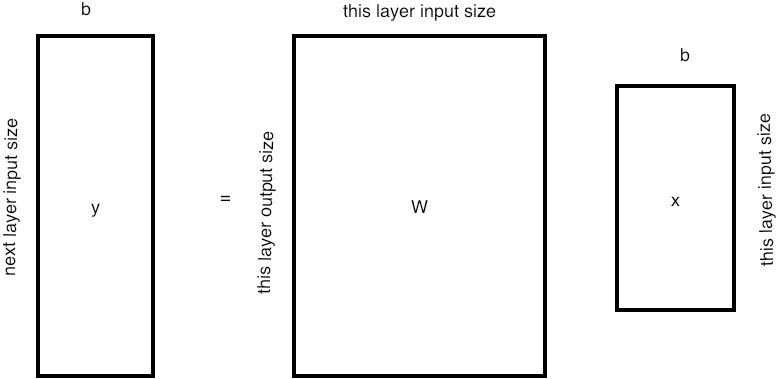
\includegraphics[scale=.4]{layershape}
  \caption{Shapes of arrays in a single layer.}
  \label{fig:layershape-seq}
\end{figure}

We picture this in figure~\ref{fig:layershape-seq}:
\begin{itemize}
\item the input batch and output batch consist of the same number of vectors;
\item the weight matrix $W$ has a number of rows equal to the output size,
  and a number of columns equal to the input size.
\end{itemize}

This importance of the \indextermtt{gemm} kernel
(sections \ref{sec:gemm} and~\ref{sec:goto-gemm})
has led people
to develop dedicated hardware for it.

Another approach would be to use a special form for the weights matrix.
In~\cite{Liao2019CompressingDN} approximation
by a \indextermsub{Toeplitz}{matrix} is investigated.
This has both advantages in space savings,
and in that the product can be done through an \indexac{FFT}.

\Level 1 {Parallelism in the weight matrix product}

We can now consider the efficient computation of~$\calN (x)$.
We already remarked that matrix-matrix multiplication
is an important kernel, but apart from that we can use
parallel processing.
Figure~\ref{fig:layershape-par} gives two parallelization strategies.

In the first one, batches are divided over processes
(or equivalently, multiple processes are working on
independent batches simultaneously);
We refer to this as \indexterm{data parallelism}.

\begin{figure}[ht]
  \hbox to \hsize{
    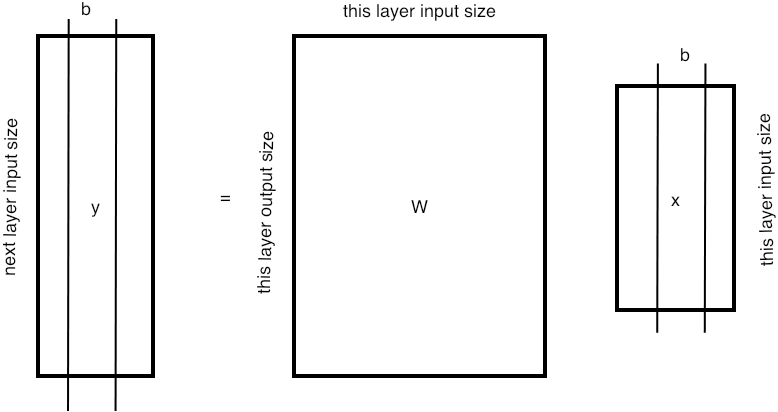
\includegraphics[scale=.25]{layershapepar}
    \hfil
  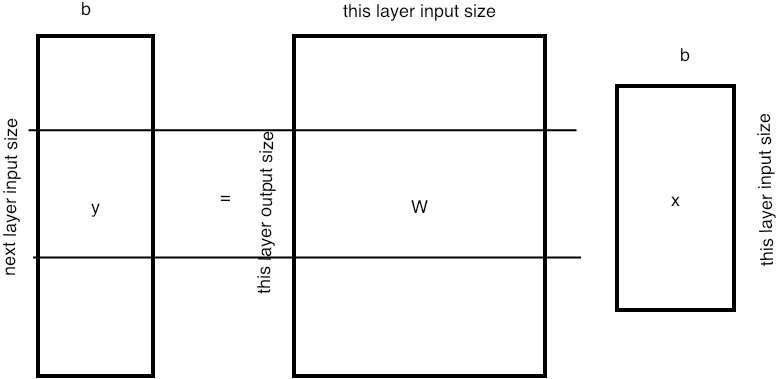
\includegraphics[scale=.25]{layershapecross}
  }
  \caption{Partitioning strategies for parallel layer evaluation.}
  \label{fig:layershape-par}
\end{figure}

\begin{exercise}
  Consider this scenario in a shared memory context. In this code:
  \begin{quote}
    \begin{tabbing}
      for \=$b=1,\ldots,\mathrm{batchsize}$\\
      \> for \=$i=1,\ldots,\mathrm{outsize}$\\
      \> \> $y_{i,b} \leftarrow \sum_j W_{i,j}\cdot x_{j,b}$\\
    \end{tabbing}
  \end{quote}
  assume that each thread computes part of the $1,\ldots,\mathrm{batchsize}$ range.

  Translate this to your favorite programming language.
  Do you store the input/output vectors by rows or columns? Why?
  What are the implications of either choice?
\end{exercise}

\begin{exercise}
  Now consider the data parallelism in a distributed memory context,
  with each process working on a slice (block column) of the batches.
  Do you see an immediate problem?
\end{exercise}

There is a second strategy,
referred to as \indexterm{model parallelism},
where the model parameters,
that is, the weights and biases, are distributed.
As you can see in figure~\ref{fig:layershape-par},
this immediately implies that output vectors
of the layer are computed distributely.

\begin{exercise}
  Outline the algorithm of this second partitioning in a distributed memory context.
\end{exercise}

The choice between these strategies depends on whether the model is large,
and the weight matrices need to be split up,
or whether the number of inputs is large.
Of course, a combination of these can also be made,
where both the model and batches are distributed.

\Level 1 {Weights update}

The calculation of the weights update
\[ \Delta W\supell \leftarrow \delta\supell {a\supellm}^t \]
is an \indexterm{outer product} of rank~$b$.
It takes two vectors, and computes a low-rank matrix from them.

\begin{exercise}
  Discuss the amount of (potential) data reuse in this operation,
  depending on the relation between $n_\ell$ and~$b$.
  Assume $n_{\ell+1}\approx n_\ell$ for simplicity.
\end{exercise}

\begin{exercise}
  Discuss the structure of the data movement involved,
  in both of the partitioning strategies of figure~\ref{fig:layershape-par}.
\end{exercise}

Apart from these aspects, 
this operation becomes even more interesting
when we consider processing mini-batches in parallel.
In that case every batch independently computes an update,
and we need to average them.
Under the assumption that each process compute a full~$\Delta W$,
this becomes an \emph{all-reduce}\index{all-reduce!in Deep Learning}.
This application of `HPC techniques' was developed
into the \indexterm{Horovod}
software~\cite{Gibiansky:baidu-allreduce,sergeev2018horovod,horovod-ai}.
In one example, considerable speedup was shown on a configuration involving
40~\acp{GPU}.

Another option would be delaying updates,
or performing them asynchronously.

\begin{exercise}
  Discuss implementing delayed or asynchronous updates in MPI.
\end{exercise}

\Level 1 {Pipelining}

A final type of parallelism can be achieved by applying pipelining over the layers.
Sketch how this can improve the efficiency of the training stage.

\Level 1 {Convolutions}

Applying a convolution is equivalent to multiplying by a \indextermsub{Toeplitz}{matrix}.
This has a lower complexity than a fully general matrix-matrix multiplication.

% \cite{Liao:DLtoeplitz}

\Level 1 {Sparse matrices}

The weights matrix can be sparsified by ignoring small entries.
This makes the
\emph{sparse matrix times dense matrix}\index{matrix!sparse!times dense matrix}
product the dominant operation~\cite{Gale:SparseDL-sc20}.

\Level 1 {Hardware support}

From the above, we conclude the importance of the \indextermtt{gemm}
computational kernel.
Dedicating a regular CPU exclusively to this purpose
is a considerable waste of silicon and power.
At the very least, using \acp{GPU} is an energy-efficient solution.

However, even more efficiency can be attained by using special purpose hardware.
Here is an overview:
\url{https://blog.inten.to/hardware-for-deep-learning-part-4-asic-96a542fe6a81}
In a way, these special purpose processors are a re-incarnation of
\indexterm{systolic array}s.

\Level 1 {Reduced precision}
\label{sec:dl-bfloat}

See section~\ref{sec:arith-bfloat}.

\Level 0 {Stuff}

\begin{quotation}
  \textsl{Universal Approximation Theorem}%
  \index{universal approximation theorem}

  Let $\varphi(\cdot)$ be a nonconstant,bounded, and
  monotonically-increasing continuous function. Let $I_m$ denote the
  $m$-dimensional unit hypercube $[0,1]^m$. The space
  of continuous functions on $I_m$ is denoted by
  $C(I_m)$. Then, given any function $f\in C(I_m)$
  and $\varepsilon>0$, there exists an integer
  $N$, real constants $v_i,b_i\in\mathbb{R}$ and
  real vectors $w_i \in \mathbb{R}^m$, where
  $i=1,\cdots,N$, such that we may define:
  \[
  F( x ) =
  \sum_{i=1}^{N} v_i \varphi \left( w_i^T x + b_i\right)
  \]
  as an approximate realization of the function $f$ where
  $f$ is independent of $\varphi$; that is,
  \[
  | F( x ) - f ( x ) | < \varepsilon
  \]
  for all $x\in I_m$. In other words, functions of the form
  $F(x)$ are dense in $C(I_m)$.
\end{quotation}

\begin{quotation}
  Can a NN approximate multiplication?

  \url{https://stats.stackexchange.com/questions/217703/can-deep-neural-network-approximate-multiplication-function-without-normalizatio}

  Traditional neural network consists of linear maps and Lipschitiz activation function. As a composition of Lischitz continuous functions, neural network is also Lipschitz continuous, but multiplication is not Lipschitz continuous. This means that neural network cannot approximate multiplication when one of the x or y goes too large.
\end{quotation}
